\newpage
\section{Processes}
\subsection{Process Concept}
\subsubsection{Concept}
又称 jobs/tasks/process. Process是一个运行的实例. 

A process includes:
\begin{itemize}
    \item text section (code, 代码段)
    \item data section (global vars, 数据段)
    \item stack (function parameter, local vars, return addresses, 栈)
    \item heap (dynamically allocated memory, 堆)
\end{itemize}

heap增长需要 OS 操作, stack 是已分配的一块空间, 在其内增长, 超过触发 stack overflow. stack 与 heap 之间的区域称为 hole, 占据超过 90\% 的空间. 

\begin{figure}[!htb]
    \centering
    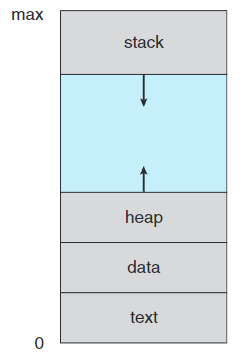
\includegraphics[width=0.22\textwidth]{pic/OS3/Layout of a process in memory.png}
    \caption{Layout of a process in memory}
\end{figure}

\subsubsection{Process State}
As a process executes, it changes state:
\begin{itemize}\small
    \item new: The process is being created
    \item running: Instructions are being executed
    \item waiting: The process is waiting/blocked for some event to occur
    \item ready: The process is waiting to be assigned to a processor
    \item terminated: The process has finished execution
\end{itemize}

\begin{figure}[!htb]
    \centering
    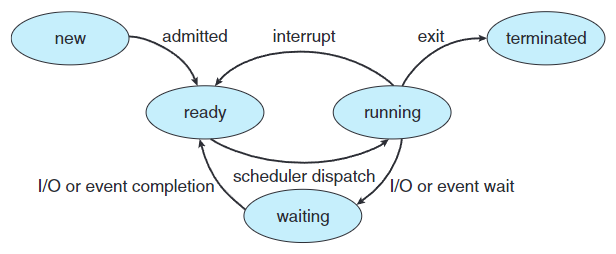
\includegraphics[width=0.42\textwidth]{pic/OS3/Diagram of process state.png}
    \caption{Diagram of process state transition}
\end{figure}
即使cpu空闲仍会有 idle 进程 一直在运行, 所以无论如何都需要 ready 缓冲. 

\subsubsection{Process Control Block (PCB)}
Information associated with each process: 
\begin{itemize}
    \item Process state
    \item Program counter
    \item Contents of CPU registers
    \item CPU scheduling information
    \item Memory-management information
    \item Accounting information
    \item I/O status information
\end{itemize}
这些由PCB存储.

\begin{figure}[!htb]
    \centering
    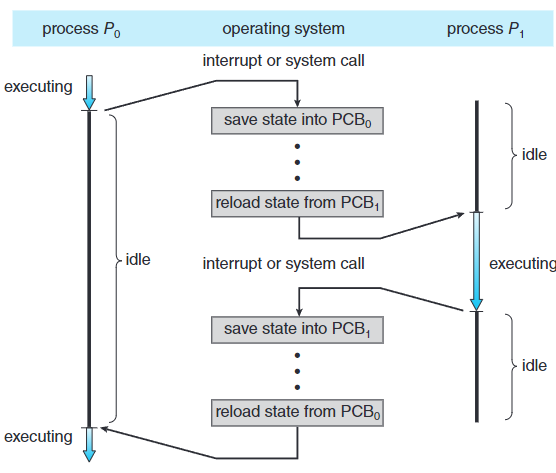
\includegraphics[width=0.42\textwidth]{pic/OS3/Diagram showing context switch from process to process}
    \caption{Diagram showing context switch from process to process}
\end{figure}
二者idle 相交称为 overhead, 是为了 multiprocessing 留的冗余. 

\subsection{Process Scheduling}
\begin{itemize}
    \item Job queue --- set of all processes in the system
    \item Ready queue --- set of all processes residing in main memory, ready and waiting to execute
    \item Device queues --- set of processes waiting for an I/O device
\end{itemize}
Processes migrate among the various queues. 一个 process 仅能在一个 queue 中. 

\subsubsection{Schedulers}
\begin{itemize}
    \item Long-term scheduler (or job scheduler) (过时了, 现在由用户决定, 是 user scheduler) --- selects which processes should be brought into memory (the ready queue). 控制着 the degree of multiprogramming. 
    \item Short-term scheduler (or CPU scheduler) --- selects which process should be executed next and allocates CPU. 频繁触发, 为了保证系统的交互性. 
\end{itemize}
UNIX and Windows do not use long-term scheduling

\paragraph{Medium Term Scheduling} 需要时将 PCB 写入磁盘 (swap out), 然后合适时恢复PCB到ready queue (swap in). 

Processes can be described as either:
\begin{itemize}
    \item I/O-bound process (IO绑定进程) --- spends more time doing I/O than
    computations, many short CPU bursts
    \item CPU-bound process (CPU绑定进程) --- spends more time doing
    computations; few very long CPU bursts
\end{itemize}


% \subsection{Operations on Processes}
% \subsection{Cooperating Processes}
% \subsection{Interprocess Communication}
% \subsection{Communication in Client-Server Systems}